%% A simple template for a lab or course report using the Hagenberg setup
%% with the standard LaTeX 'report' class
\documentclass[english,11pt]{report}		
%\documentclass[ngerman,11pt]{report}
\usepackage{hyperref}
\usepackage{hgb}
\usepackage{hgbbib}
\usepackage{hgbheadings}
\usepackage{tabu}
\usepackage{caption}
\usepackage{chronology}
\usepackage[topmargin=.5 in]{geometry}
\graphicspath{{images/}}   % where are the images?
\bibliography{literatur}  % requires literatur.bib 
\title{\huge{Study of the Electrical system of the new Power and Blowing Station II}\\[.4em]
\small{and}\\[.4em]
\huge{Emergency calculations for power requirements in case of power failure} \\[1em] \Large{Himanshu Gupta} \\
\Large{Ishaan Dewangan} \\
\Large{Mihir Kumar} \\
\Large{Anshul Dubey} \\
\Large{Salil Jain} \\
[2em] \large{Mid-Sem Report submitted in partial fulfillment for\\
Practice School I (BITS F221)\\[1em]
under the guidance of\\[.3em]}
\Large{Mr. V.S. Dewangan}\\[.8em]
\large{Submitted to}\\[.3em]
\Large{Prof. Ashutosh Bhatia}}
\date{$25^{th}$ June 2017}

% \lhead{
\includegraphics[width=1cm]{bits123.png}}
% \lhead{
\includegraphics[width=1.5cm]{sail123.png}}
%%%----------------------------------------------------------
\begin{document}
%%%----------------------------------------------------------
\maketitle

\tableofcontents

\chapter{Project Overview}

\section{What is the project about?}

\begin{itemize}
\item To study of all electrical and mechanical system of PBS-2
\item Calculation of the emergency power requirement of different units of PBS-2.
\item Identification of the source of power in BSP to ensure emergency supply in case of power failure.
\end{itemize}

\section{Objective and Significance of the project}

\begin{itemize}
\item Detailed exposure of various process involved in power generation system in steel industry.
\item Function of boilers , DM water plant ,cooling water pump house , cooling towers , turbine, generator for power requirement in any industry .
\item Learning of the various control systems in power plant operations .
\item Role of SCADA  in electrical control system and communication.
\item Calculation of the emergency power requirements of the new Power and Blowing Station II which is being installed in BSP 
\item Power generation from waste heat of COB-11 is also envisaged in this project and 4 MW along with process steam is being utilized in BSP.
\item Total electrical system of BSP are interlinked with PBS-2 for reliable operation of power system in case of power failure
\end{itemize}

\pagebreak
\section{Learning outcomes and Expected Knowledge gain and Deliverable from the project}
% \markboth{}{}
\begin{itemize}
\item Exposure to all electrical system in power industry like generator reactor HT breaker  , LT breaker transformer  cable sizing etc. 
\item Detailed study of SLD for power requirement in any industry 
\item Project management for execution of any project 
\item Commissioning methodology of electrical system 
\item Power calculation of any upcoming unit for reliable operation of plant 
\item Exposure to power plant operation with detailed knowledge of each equipment
\item Introduction to DCS, PLC, SCADA for future references
\end{itemize}

\section{Current Status}
\begin{itemize}
\item The field work has been going on and the detailed study of different units involved in PBS-2 have been made
\item The Project is on schedule
\end{itemize}

\section{Site Map}
\includegraphics[width =6in]{siteimg.png}

\section{Project Packages}
\begin{center}
\begin{tabu}to 0.8\textwidth { | X[l] | X[l] | X[l] | X[l]|} 
\hline
Package & Installation & Contractors & Contract signing date \\
\hline
011-01-A & 3 Boilers and its auxiliaries. STB Building along with EOT crane  & M/s Fujian Longking Corporation Ltd. and M/s Allied Engineering Services Pvt. Ltd. & 24.03.12\\
\hline
011-01-B & 25 MW STG, 4 MW BPTG, Cooling Tower, Pump House & M/s Triveni Engineering and Industries Ltd.,Banglore & 19.01.12\\
\hline
011-01-C & 3X 225 M3 /Hr. DM water Plant & M/s TechnoFab Engineering Ltd., New Delhi
 & 25.02.12 \\
\hline
12 & 3 STB's and its auxiliaries. & Bharat Heavy Electricals Ltd. & 11.11.10\\
\hline
\end{tabu}
\end{center}

\chapter{Boiler}
Boilers or Steam generators are used to generate steam at desired rate and desired pressure
and temperature by burning fuel in its furnace. They can be classified as fire tube or water tube
boilers depending on whether the hot gas or water is present in the tubes inside the boiler.\\

\section{Types of Boilers}
\textbf{Fire Tube Boilers}\\
Earlier designs include fire tube boilers suitable for small steam requirements. They can be
externally fired or internally fired. The externally fired is the one in which furnace is outside the boiler shell. The products of combustion flow through the tubes which are immersed in a shell
containing water As the flue gases flow through the tubes, heat is transferred from gas to water
and water is converted to steam. In internally fired fire tube boiler, the furnace is present inside the shell containing water. Combustion gases flow through the pipes and let out to the
atmosphere. These gases exchange the heat with the water present in the shell. The major
shortcoming of fire tube boiler is that the pressure limitations are inherent in its basic design.
The steam present in the drum exerts hoop stress on the shell and larger the shell, larger is the
stresses induced and to increase the pressure carrying capacity, the thickness has to be
increased which increases the manufacturing cost.\\[1em]
\textbf{Water Tube Boilers}\\
Modern boilers are mostly water tube boilers. These were developed to permit increases in
boiler capacity with reasonable metal stresses. Since water tube boilers have water flowing in
small tubes, the pressure carrying capacity of the tubes being higher, they are used to generate
high pressure steam. The water tube boilers can be further divided as straight tube or bent tube
boilers.\\
\section{How does a Boiler work}
\textbf{Economizer} is the first step in the steam generation process. The feed water from the boiler feed pump enters the economizer where it is heated by the hot flue gases. The hot flue gases
leave burner and travel through the furnace to the chimney and exchanges its heat from
different heat ex-changers in its way to the exhaust chimneys.\\[1em]
After getting saturated, the feed water is taken to the \textbf{Boiler drum}. The purpose of boiler drum is to evaporate the feed water or provide latent heat. The saturated water from the boiler drum comes down via \textbf{Downcommers} and is then passed through \textbf{water walls (Risers)} which are number of evaporation tubes spaced all around the walls of the furnace and is used to take away the latent heat using the heat exchange from the hot flue gases. The flow of the feed
water can be natural circulation by the density difference between the water in the riser and
downcommers or when the pressure is higher, the circulation pump is used to provide the flow
as the density difference is not enough to cause natural circulation. The mixture of saturated
liquid and steam then enters again to boiler drum where the steam and the liquid are separated
and the steam goes to the superheaters.\\[1em]
A \textbf{Superheater} is a heat exchanger in which heat is transferred in a saturated steam to increase its temperature to the desired value. In modern boilers, more than 40\% of the heat absorption takes place in superheaters. Superheaters are commonly classified as either convective, radiant or pendant supreheaters. The \textbf{Convective superheaters} are often termed as primary
superheaters where the saturated steam from the drum is admitted. After passing through the
convective superheater, the steam proceeds to the Radiant superheaters where the heat
exchange between the flue gases and the steam is mostly due to radiation. As the heat
exchange is due to radiation, the amount of temperature increase is generally more than what
is required so the steam is desuperheated in \textbf{Desuperheaters}. The desuperheater is a direct
contact type and the tapping from the boiler feed water is taken and sprayed over the steam to
desuperheat it. The steam is then passed to \textbf{Pendant superheater} where the steam is finally
heated to the desired temperature. There heat is transferred partly by convection and partly by
radiation.\\[1em]
The flue gases are produced in the burners by burning the mixture of gases and preheated air.
The gases contain mixture of BF (Blast Furnace gas), CO (Coke oven) gas, LDO (Light diesel oil)
gas. The air is preheated using the \textbf{Air Preheater}. The air is sucked through the \textbf{Forced draught} fan and then passed through the Air Preheater where the heat exchange takes place between the flue gases and the air.\\[1em]
The flue gases after passing through the air perheater then passes through the \textbf{Electrostatic Precipitator} where the dust particles are precipitated and the \textbf{Induced Draught}. Fan then takes
it to the atmosphere via \textbf{chimneys}.

\section{Specifications of Boiler in PBS – 2}
\begin{center}
\begin{tabular} { | c | c |} 
\hline
Heating area of Economizer&3100 m^2\\ \hline
Heating area of Superheater&967 m^2\\ \hline
Heating area of Water walls&1005 m^2\\ \hline
Heating area of Evaporators&1240 m^2\\ \hline
Total heating area&6312 m^2\\ \hline
Rated capacity&150 T/hr, 383 Mpa, 450$^{\circ}$C\\ \hline
&\\ \hline
\textbf{Design Fuel :}  & \\ \hline
BF Gas & 3245KJ/Nm^3 \\ \hline
BOF Gas & 7531 KJ/Nm^3 \\ \hline
CO Gas & 16246 KJ/Nm^3 \\ 
\hline
\end{tabular}
\end{center}

\section{Flow Diagram of Boiler}
\begin{center}
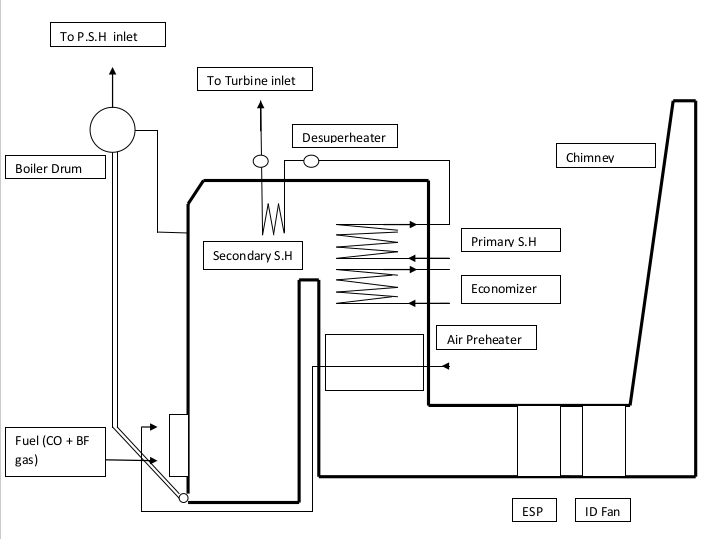
\includegraphics[width =5in]{flow}
\end{center}
    


\chapter{STG 25 MW}
\section{Process Flow Diagram}
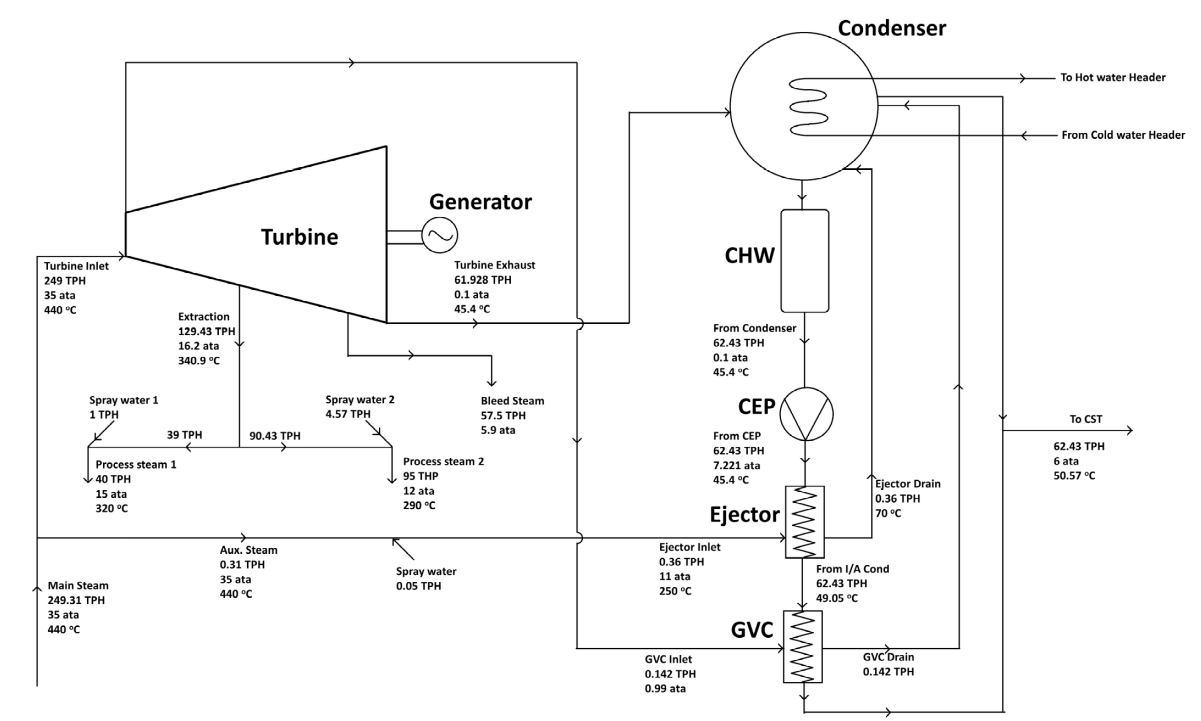
\includegraphics[width =6in]{stgprocessflow.png}
\section{Electrical Equipment}
\begin{center}
\begin{tabular} { | c | c | c |} 
\hline
Equipment & Specification & Location \\ \hline
Transformers & 36MVA, 11kV/6.9kV & 0 meters B-C \\ \hline
Breakers & 1.3150 Amp, 2.2000 Amp & 11 meters A-B \\ \hline
Reactor & 1500 Amp, 12\% & 3 meters A-B \\ \hline
DCS &  & 11 meters \\ \hline
LT Panels & & 11 meters\\  
\hline
\end{tabular}
\end{center}
\section{STG 25 MW Electrical Component}
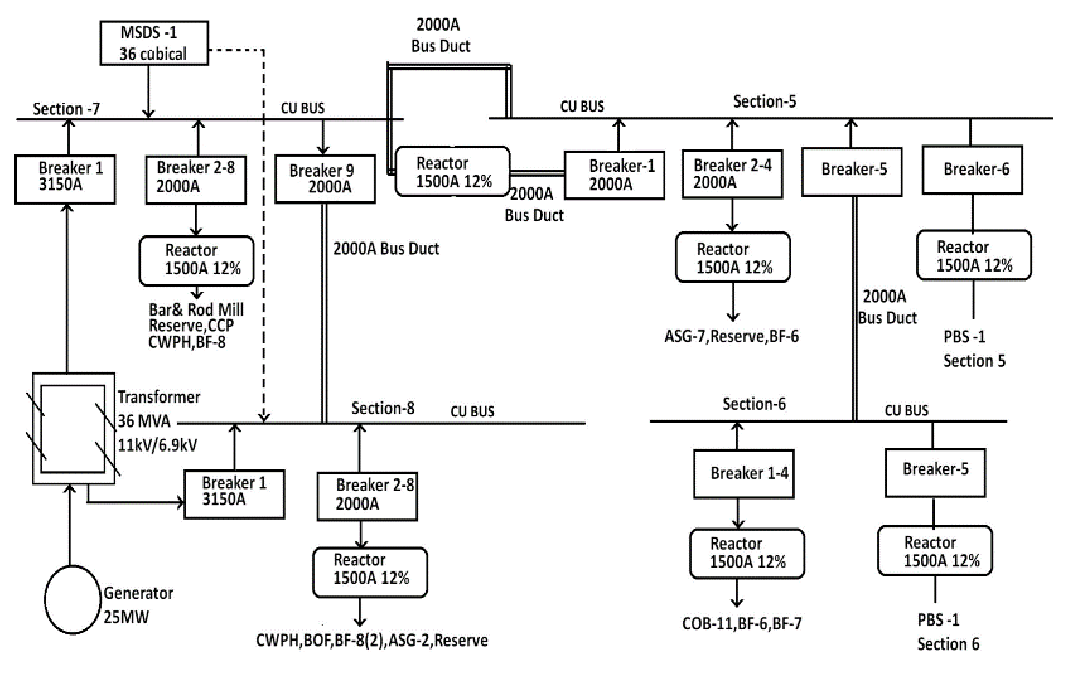
\includegraphics[width =6in]{stg25mw}
\section{STG - Electrical Reserve Supply Switch Board}
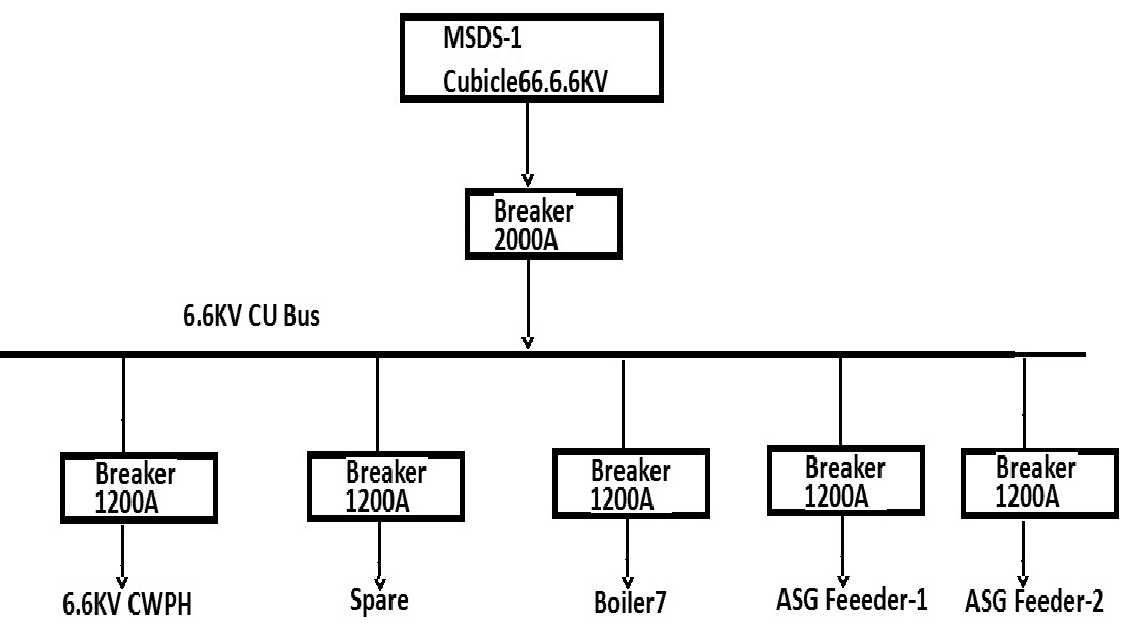
\includegraphics[width =6in]{stgelec}   

\chapter{Cooling Tower and Pump House}
\section{Overview}
Cooling towers are the devices that take heat from the cooling water to cool them for condenser heat removal. The heat is rejected to the atmosphere. The cooling towers can be further divided as Wet type and Dry type.
\subsection{Wet Cooling towers}
Wet cooling tower have showers that sprays hot water over horizontal packing. The outside
air enters the tower through louvers on the side of the tower. The water evaporated is
directly proportional to cooling. Cold water is collected in a concrete basin and is pumped
again to the condensers.\\[1em]
The minimum temperature to which water can be cooled is the adiabatic saturation or wet
bulb temperature of the ambient air. At this temperature, the air is 100 % saturated and
cannot absorb more moisture.\\[1em]
A Cooling tower is specified by
$$Approach(A) = (Exit \,Temperature \,of \,C.W.) - (WBT \,of \,ambient \,air)$$
where C.W. stands for Cooling Tower and WBT stands for Wet Bulb temperatue which is the temperature a parcel of air would have if it were cooled to saturation (100\% relative humidity) by the evaporation of water into it, with the latent heat being supplied by the parcel.\\[1em]
Also the cooling efficiency is defined as
$$\eta = \frac{Actual \,Cooling}{Maximum \,possible \,Cooling}$$
We have 10 cooling cells with 9 working and 1 standby. Temperature reduces from 42$^{\circ}$ to 34$^{\circ}$ at supplied to STG and STB condensor. Its cooling capacity is 19655 m$^3$/hr. It has 5 vertical axial flow pumps with 3 working and 2 for standby. Water sump in pump house is 8.5 m deep.
\section{Diagram}
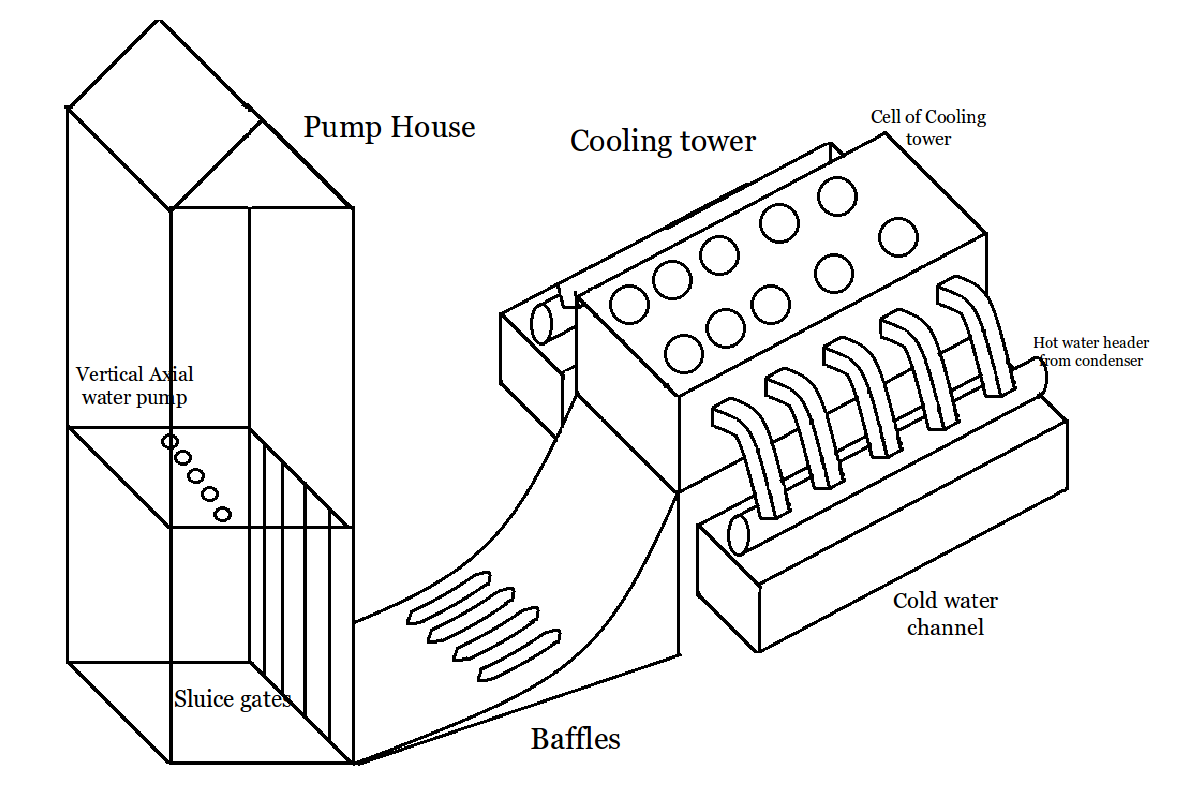
\includegraphics[width =6in]{cooling}

\chapter{STB}
\section{Process Overview of STB and Auxiliaries}
The steam used to drive the blowers is produced in \textbf{3 Boilers} at 40 ata, 450 degree Celsius. Waste gases from blast furnace and coke oven mainly BF gas and CO gas are used to fire the
burners in boiler to produce steam. The steam so produced is sent to main steam header from
where tapings are taken for different stations mainly \textbf{Turbo blowers, Turbo generators and
Pressure Reducing and De superheating Station}.\\[1em]
Steam enters the \textbf{Turbine} at around 36 ata, 440 degree Celsius. The steam in turbine passes
through different stages where its enthalpy is converted into rotational energy to drive the
turbine shaft which in turn drives the \textbf{Blower} attached. The blower thus sucks the air passing through air filtration system and delivers the high pressure air to the blower outlet. The steam from turbine outlet goes through \textbf{Condenser} where it is condensed by cooling water to liquid condensate which is collected in hotwell.\\[1em]
The liquid condensate from the hotwell is then pumped using \textbf{Condensate Extraction Pump}.
The condensate is then passed through the \textbf{Steam Jet Air Ejector} where the condensate is
heated and the air in the condenser is simultaneously ejected using the steam from \textbf{PRDS}. The condensate is then passed through the \textbf{Gland Steam Condenser} where it is heated using the PRDS steam.\\[1em]
The condensate is then stored in the \textbf{Condensate Storage Tank}. The condensate is then
transferred to the \textbf{Dearator} using the \textbf{Condensate Transfer Pump}. The condensate is sprayed from the top in the dearator and PRDS steam is used to heat the condensate and remove the
impurities. The feed water so formed is collected and then pumped to the Boiler using the
\textbf{Boiler Feed Pump}. The feedwater in boiler is first converted to saturated liquid by
economizer and then it goes to the boiler drum where it is evaporated and then passes through
superheater before reaching its final state and transferred to main steam header.
\section{Layout of STB PBS-2}
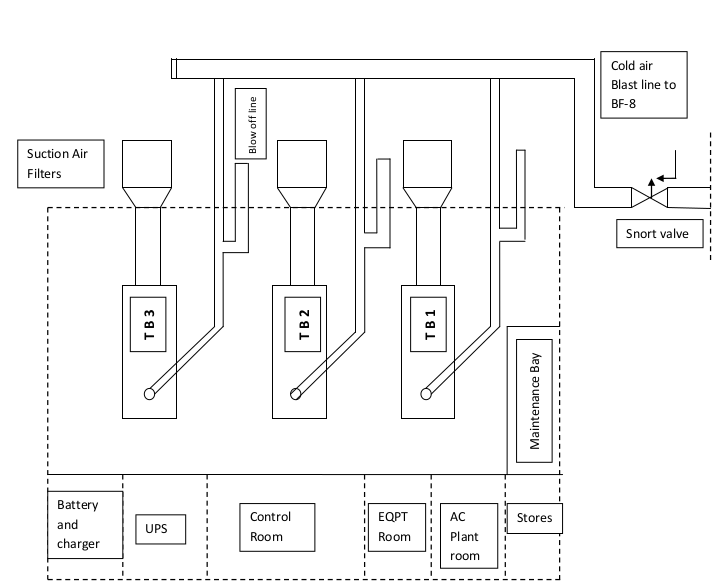
\includegraphics[width =6in]{layoutstb}
\section{Air Distribution system STB PBS-2}
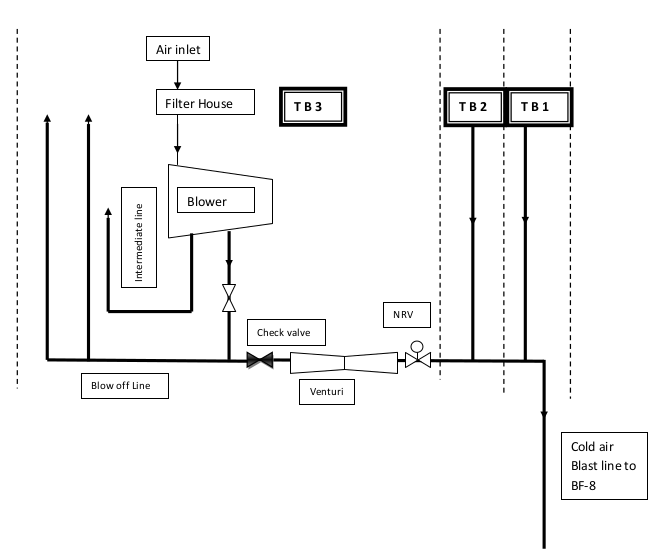
\includegraphics[width =6in]{airstb}
\chapter{Timeline Ahead}
\begin{tikzpicture}[snake=zigzag, line before snake = 5mm, line after snake = 5mm]
% draw horizontal line   
\draw (-2,0) -- (14,0);


% draw vertical lines
\foreach \x in {0,4,8,12}
  \draw (\x cm,3pt) -- (\x cm,-3pt);

% draw nodes
% \draw (0,0) node[below=3pt] {$ 0 $} node[above=3pt] {$   $};
% \draw (1,0) node[below=3pt] {$ 1 $} node[above=3pt] {$ 10 $};
% \draw (2,0) node[below=3pt] {$ 2 $} node[above=3pt] {$ 20 $};
\draw (0,0) node[below=3pt] {$ 22^{nd} June $} node[above=3pt] {$ covering \,BPTG $};
% \draw (4,0) node[below=3pt] {$ 5 $} node[above=3pt] {$ 50 $};
\draw (4,0) node[below=3pt] {$ covering \,STB $} node[above=3pt] {$ 24^{th} June $};
\draw (8,0) node[below=3pt] {$ 26^{th} June $} node[above=3pt] {$ Start \,Calculations $};
\draw (12,0) node[below=3pt] {$ Verifying \,the \,calculations $} node[above=3pt] {$ 30^{th} June $};
\end{tikzpicture}
\\[5em]
\begin{center}
\textbf{\textit{The end}}
\end{center}

\end{document}
